\documentclass{standalone}
\usepackage{tikz}
\usetikzlibrary{patterns, positioning}
\usepackage[sfdefault]{ClearSans} %% option 'sfdefault' activates Clear Sans as the default text font
\usepackage[T1]{fontenc}

\begin{document}
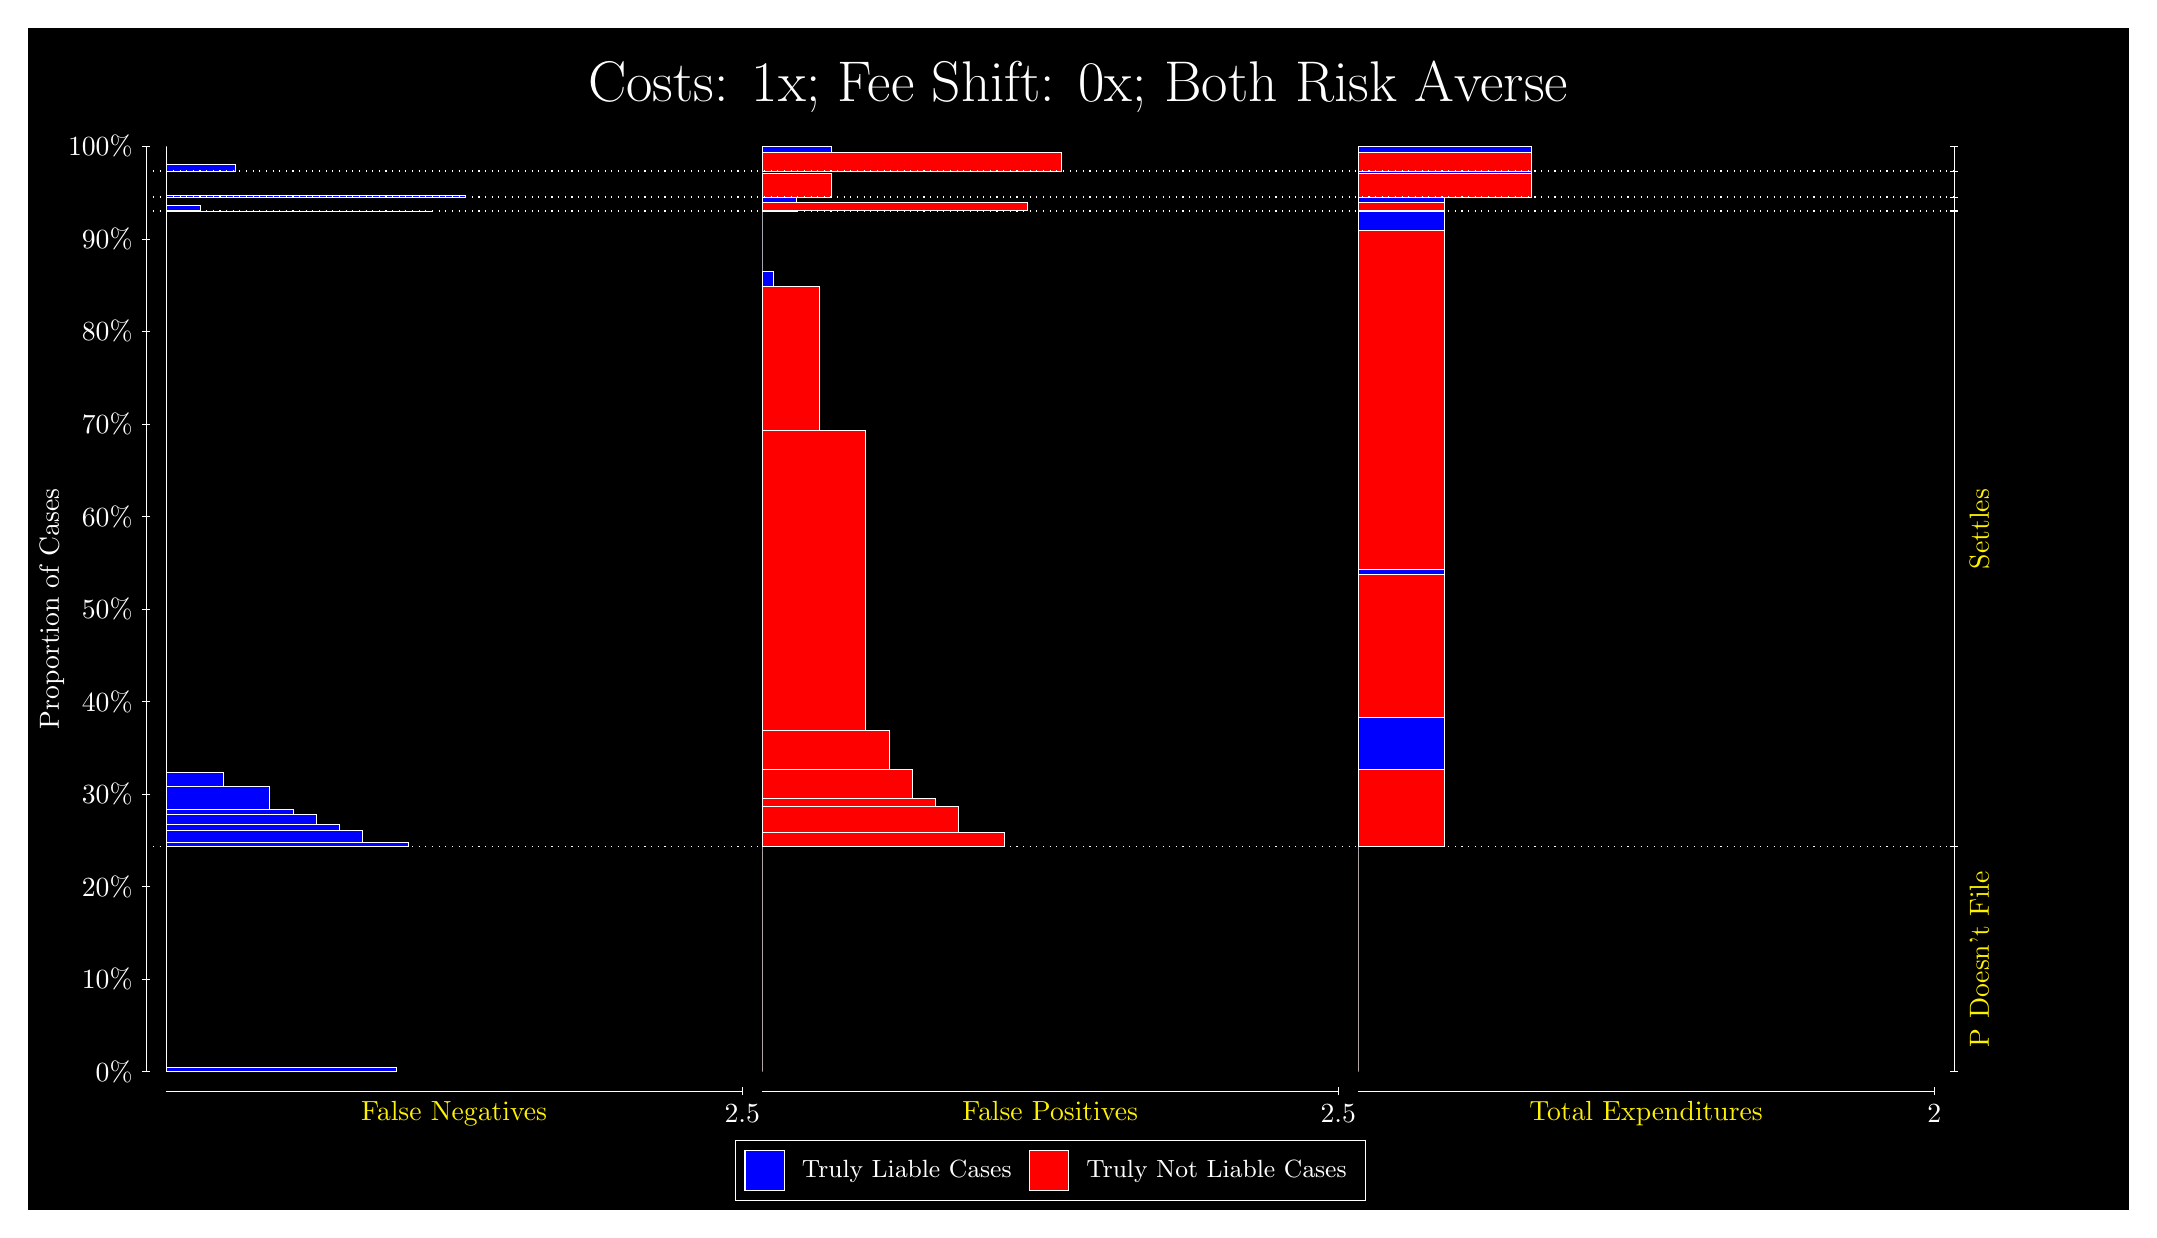
\begin{tikzpicture}
\draw[fill=black] (0,0) rectangle (26.667,15);
\draw[text=white] (0,13.5) rectangle (26.667,15) node[midway] {\huge Costs: 1x; Fee Shift: 0x; Both Risk Averse};
\draw[white, very thin] (1.5,1.75) -- (1.5,13.5);
\node[rotate=90, text=white, anchor=center] at (0.3, 7.625) {Proportion of Cases};
\draw[white, very thin] (1.45,1.75) -- (1.55,1.75);
\node[text=white, anchor=east] at (1.45, 1.75) {0\%};
\draw[white, very thin] (1.45,2.925) -- (1.55,2.925);
\node[text=white, anchor=east] at (1.45, 2.925) {10\%};
\draw[white, very thin] (1.45,4.1) -- (1.55,4.1);
\node[text=white, anchor=east] at (1.45, 4.1) {20\%};
\draw[white, very thin] (1.45,5.275) -- (1.55,5.275);
\node[text=white, anchor=east] at (1.45, 5.275) {30\%};
\draw[white, very thin] (1.45,6.45) -- (1.55,6.45);
\node[text=white, anchor=east] at (1.45, 6.45) {40\%};
\draw[white, very thin] (1.45,7.625) -- (1.55,7.625);
\node[text=white, anchor=east] at (1.45, 7.625) {50\%};
\draw[white, very thin] (1.45,8.8) -- (1.55,8.8);
\node[text=white, anchor=east] at (1.45, 8.8) {60\%};
\draw[white, very thin] (1.45,9.975) -- (1.55,9.975);
\node[text=white, anchor=east] at (1.45, 9.975) {70\%};
\draw[white, very thin] (1.45,11.15) -- (1.55,11.15);
\node[text=white, anchor=east] at (1.45, 11.15) {80\%};
\draw[white, very thin] (1.45,12.325) -- (1.55,12.325);
\node[text=white, anchor=east] at (1.45, 12.325) {90\%};
\draw[white, very thin] (1.45,13.5) -- (1.55,13.5);
\node[text=white, anchor=east] at (1.45, 13.5) {100\%};

\draw[white, very thin] (24.457,1.75) -- (24.457,13.5);
\draw[white, very thin] (24.407,1.75) -- (24.507,1.75);
\node[anchor=west] at (24.407, 1.75) {};
\draw[white, very thin] (24.407,4.6045) -- (24.507,4.6045);
\node[anchor=west] at (24.407, 4.6045) {};
\draw[white, very thin] (24.407,12.672) -- (24.507,12.672);
\node[anchor=west] at (24.407, 12.672) {};
\draw[white, very thin] (24.407,12.685) -- (24.507,12.685);
\node[anchor=west] at (24.407, 12.685) {};
\draw[white, very thin] (24.407,12.857) -- (24.507,12.857);
\node[anchor=west] at (24.407, 12.857) {};
\draw[white, very thin] (24.407,13.186) -- (24.507,13.186);
\node[anchor=west] at (24.407, 13.186) {};
\draw[white, very thin] (24.407,13.5) -- (24.507,13.5);
\node[anchor=west] at (24.407, 13.5) {};

\draw[white, very thin, fill=blue] (1.75,1.75) rectangle (4.6775,1.8006);
\draw[white, very thin, fill=red] (1.75,1.8006) rectangle (1.75,4.6045);
\draw[white, very thin, fill=blue] (1.75,4.6045) rectangle (4.8239,4.6631);
\draw[white, very thin, fill=blue] (1.75,4.6631) rectangle (4.2384,4.813);
\draw[white, very thin, fill=blue] (1.75,4.813) rectangle (3.9457,4.8959);
\draw[white, very thin, fill=blue] (1.75,4.8959) rectangle (3.6529,5.0189);
\draw[white, very thin, fill=blue] (1.75,5.0189) rectangle (3.3602,5.0817);
\draw[white, very thin, fill=blue] (1.75,5.0817) rectangle (3.0674,5.37);
\draw[white, very thin, fill=blue] (1.75,5.37) rectangle (2.4819,5.555);
\draw[white, very thin, fill=red] (1.75,5.555) rectangle (1.75,12.672);
\draw[white, very thin, fill=blue] (1.75,12.672) rectangle (5.1167,12.673);
\draw[white, very thin, fill=red] (1.75,12.673) rectangle (1.75,12.685);
\draw[white, very thin, fill=blue] (1.75,12.685) rectangle (2.1891,12.752);
\draw[white, very thin, fill=red] (1.75,12.752) rectangle (1.75,12.857);
\draw[white, very thin, fill=blue] (1.75,12.857) rectangle (5.5558,12.883);
\draw[white, very thin, fill=red] (1.75,12.883) rectangle (1.75,13.186);
\draw[white, very thin, fill=blue] (1.75,13.186) rectangle (2.6283,13.266);
\draw[white, very thin, fill=red] (1.75,13.266) rectangle (1.75,13.5);
\draw[white, very thin, fill=red] (9.3189,1.75) rectangle (9.3189,4.5539);
\draw[white, very thin, fill=blue] (9.3189,4.5539) rectangle (9.3189,4.6045);
\draw[white, very thin, fill=red] (9.3189,4.6045) rectangle (12.393,4.7832);
\draw[white, very thin, fill=red] (9.3189,4.7832) rectangle (11.807,5.1147);
\draw[white, very thin, fill=red] (9.3189,5.1147) rectangle (11.515,5.2177);
\draw[white, very thin, fill=red] (9.3189,5.2177) rectangle (11.222,5.5848);
\draw[white, very thin, fill=red] (9.3189,5.5848) rectangle (10.929,6.0804);
\draw[white, very thin, fill=red] (9.3189,6.0804) rectangle (10.636,9.8989);
\draw[white, very thin, fill=red] (9.3189,9.8989) rectangle (10.051,11.722);
\draw[white, very thin, fill=blue] (9.3189,11.722) rectangle (9.4652,11.907);
\draw[white, very thin, fill=blue] (9.3189,11.907) rectangle (9.3189,12.672);
\draw[white, very thin, fill=red] (9.3189,12.672) rectangle (9.758,12.684);
\draw[white, very thin, fill=blue] (9.3189,12.684) rectangle (9.3189,12.685);
\draw[white, very thin, fill=red] (9.3189,12.685) rectangle (12.686,12.79);
\draw[white, very thin, fill=blue] (9.3189,12.79) rectangle (9.758,12.857);
\draw[white, very thin, fill=red] (9.3189,12.857) rectangle (10.197,13.16);
\draw[white, very thin, fill=blue] (9.3189,13.16) rectangle (9.3189,13.186);
\draw[white, very thin, fill=red] (9.3189,13.186) rectangle (13.125,13.42);
\draw[white, very thin, fill=blue] (9.3189,13.42) rectangle (10.197,13.5);
\draw[white, very thin, fill=red] (16.888,1.75) rectangle (16.888,4.5539);
\draw[white, very thin, fill=blue] (16.888,4.5539) rectangle (16.888,4.6045);
\draw[white, very thin, fill=red] (16.888,4.6045) rectangle (17.986,5.5848);
\draw[white, very thin, fill=blue] (16.888,5.5848) rectangle (17.986,6.2439);
\draw[white, very thin, fill=red] (16.888,6.2439) rectangle (17.986,8.067);
\draw[white, very thin, fill=blue] (16.888,8.067) rectangle (17.986,8.1256);
\draw[white, very thin, fill=red] (16.888,8.1256) rectangle (17.986,12.44);
\draw[white, very thin, fill=blue] (16.888,12.44) rectangle (17.986,12.672);
\draw[white, very thin, fill=red] (16.888,12.672) rectangle (17.986,12.684);
\draw[white, very thin, fill=blue] (16.888,12.684) rectangle (17.986,12.685);
\draw[white, very thin, fill=red] (16.888,12.685) rectangle (17.986,12.79);
\draw[white, very thin, fill=blue] (16.888,12.79) rectangle (17.986,12.857);
\draw[white, very thin, fill=red] (16.888,12.857) rectangle (19.083,13.16);
\draw[white, very thin, fill=blue] (16.888,13.16) rectangle (19.083,13.186);
\draw[white, very thin, fill=red] (16.888,13.186) rectangle (19.083,13.42);
\draw[white, very thin, fill=blue] (16.888,13.42) rectangle (19.083,13.5);
\draw[white, dotted] (1.5,4.6045) -- (24.457,4.6045);
\draw[white, dotted] (1.5,12.672) -- (24.457,12.672);
\draw[white, dotted] (1.5,12.685) -- (24.457,12.685);
\draw[white, dotted] (1.5,12.857) -- (24.457,12.857);
\draw[white, dotted] (1.5,13.186) -- (24.457,13.186);
\draw[white, very thin] (1.75,1.5) -- (9.0689,1.5);
\node[text=yellow, anchor=north] at (5.4094, 1.5) {False Negatives};
\draw[white, very thin] (9.0689,1.45) -- (9.0689,1.55);
\node[text=white, anchor=north] at (9.0689, 1.45) {2.5};

\draw[white, very thin] (9.3189,1.5) -- (16.638,1.5);
\node[text=yellow, anchor=north] at (12.978, 1.5) {False Positives};
\draw[white, very thin] (16.638,1.45) -- (16.638,1.55);
\node[text=white, anchor=north] at (16.638, 1.45) {2.5};

\draw[white, very thin] (16.888,1.5) -- (24.207,1.5);
\node[text=yellow, anchor=north] at (20.547, 1.5) {Total Expenditures};
\draw[white, very thin] (24.207,1.45) -- (24.207,1.55);
\node[text=white, anchor=north] at (24.207, 1.45) {2};

\node[text=yellow, centered, rotate=90] at (24.777, 3.1773) {P Doesn't File};
\node[text=yellow, centered, rotate=90] at (24.777, 8.6385) {Settles};





\draw (12.978300999999998,1.5) node[draw=none] (baseCoordinate) {};
\begin{scope}[align=center]
        \matrix[scale=0.5, draw=white, below=0.5cm of baseCoordinate, nodes={draw}, column sep=0.1cm]{
            \node[rectangle, draw, minimum width=0.5cm, minimum height=0.5cm, fill=blue] {}; &
            \node[draw=none, font=\small, text=white] (B) {Truly Liable Cases}; &
            \node[rectangle, draw, minimum width=0.5cm, minimum height=0.5cm, fill=red] {}; &
            \node[draw=none, font=\small, text=white] (B) {Truly Not Liable Cases}; \\
            };
\end{scope}

\end{tikzpicture}
\end{document}